% Options for packages loaded elsewhere
\PassOptionsToPackage{unicode}{hyperref}
\PassOptionsToPackage{hyphens}{url}
%
\documentclass[11pt,a4paper]{article}
\usepackage[a4paper,margin=2.4cm,headheight=15pt]{geometry}
\usepackage{titlesec}
\usepackage{fancyhdr}
\usepackage{caption}
\usepackage{enumitem}
\usepackage{microtype}
\usepackage{float}
\usepackage{array}
\usepackage{booktabs}
\usepackage{tabularx}
\usepackage{ragged2e}
\usepackage{lastpage}
\setlist[itemize]{leftmargin=1.5em,itemsep=3pt,topsep=4pt}
\setlist[enumerate]{leftmargin=1.7em,itemsep=3pt,topsep=4pt}
\titleformat{\section}{\Large\bfseries\color{blue!55!black}}{\thesection}{0.65em}{}[\titlerule]
\titleformat{\subsection}{\large\bfseries\color{blue!45!black}}{\thesubsection}{0.6em}{}
\titlespacing*{\section}{0pt}{2.0ex plus .5ex minus .2ex}{1.0ex}
\pagestyle{fancy}
\fancyhf{}
\fancyhead[L]{\small Customer Churn Early-Warning Dashboard}
\fancyhead[R]{\small BA6003 Final Project Report}
\fancyfoot[C]{\thepage\ of \pageref{LastPage}}
\renewcommand{\headrulewidth}{0.4pt}
\renewcommand{\footrulewidth}{0pt}
\usepackage{amsmath,amssymb}
\usepackage{iftex}
\ifPDFTeX
  \usepackage[T1]{fontenc}
  \usepackage[utf8]{inputenc}
  \usepackage{textcomp} % provide euro and other symbols
\else % if luatex or xetex
  \usepackage{unicode-math} % this also loads fontspec
  \defaultfontfeatures{Scale=MatchLowercase}
  \defaultfontfeatures[\rmfamily]{Ligatures=TeX,Scale=1}
\fi
\usepackage{lmodern}
\ifPDFTeX\else
  % xetex/luatex font selection
\fi
% Use upquote if available, for straight quotes in verbatim environments
\IfFileExists{upquote.sty}{\usepackage{upquote}}{}
\IfFileExists{microtype.sty}{% use microtype if available
  \usepackage[]{microtype}
  \UseMicrotypeSet[protrusion]{basicmath} % disable protrusion for tt fonts
}{}
\makeatletter
\@ifundefined{KOMAClassName}{% if non-KOMA class
  \IfFileExists{parskip.sty}{%
    \usepackage{parskip}
  }{% else
    \setlength{\parindent}{0pt}
    \setlength{\parskip}{6pt plus 2pt minus 1pt}}
}{% if KOMA class
  \KOMAoptions{parskip=half}}
\makeatother
\usepackage{xcolor}
\usepackage{longtable,booktabs,array}
\usepackage{calc} % for calculating minipage widths
% Correct order of tables after \paragraph or \subparagraph
\usepackage{etoolbox}
\makeatletter
\patchcmd\longtable{\par}{\if@noskipsec\mbox{}\fi\par}{}{}
\makeatother
% Allow footnotes in longtable head/foot
\IfFileExists{footnotehyper.sty}{\usepackage{footnotehyper}}{\usepackage{footnote}}
\makesavenoteenv{longtable}
\usepackage{graphicx}
\makeatletter
\def\maxwidth{\ifdim\Gin@nat@width>\linewidth\linewidth\else\Gin@nat@width\fi}
\def\maxheight{\ifdim\Gin@nat@height>\textheight\textheight\else\Gin@nat@height\fi}
\makeatother
% Scale images if necessary, so that they will not overflow the page
% margins by default, and it is still possible to overwrite the defaults
% using explicit options in \includegraphics[width, height, ...]{}
\setkeys{Gin}{width=\maxwidth,height=\maxheight,keepaspectratio}
% Set default figure placement to htbp
\makeatletter
\def\fps@figure{htbp}
\makeatother
\ifLuaTeX
  \usepackage{luacolor}
  \usepackage[soul]{lua-ul}
\else
  \usepackage{soul}
\fi
\setlength{\emergencystretch}{3em} % prevent overfull lines
\providecommand{\tightlist}{%
  \setlength{\itemsep}{0pt}\setlength{\parskip}{0pt}}
\setcounter{secnumdepth}{3} % number sections, subsections and subsubsections
\ifLuaTeX
  \usepackage{selnolig}  % disable illegal ligatures
\fi
\usepackage{bookmark}
\IfFileExists{xurl.sty}{\usepackage{xurl}}{} % add URL line breaks if available
\urlstyle{same}
\hypersetup{
  colorlinks=true,
  linkcolor=blue!45!black,
  urlcolor=blue!55!black,
  citecolor=blue!45!black,
  pdftitle={Customer Churn Early-Warning Dashboard -- Final Project Report},
  pdfcreator={LaTeX via Pandoc}}

\author{}
\date{}

\begin{document}

\begin{titlepage}
\centering
\vspace*{1.6cm}
{\Huge\bfseries\color{blue!55!black} Customer Churn\par}
\vspace{0.25cm}
{\Huge\bfseries\color{blue!55!black} Early-Warning Dashboard\par}
\vspace{0.8cm}
{\Large Final Project Report\par}
\vspace{1.0cm}
\rule{0.82\textwidth}{1pt}\par
\vspace{0.7cm}
{\large BA6003 Database \& Programming\par}
\vspace{0.25cm}
{\large 14 October 2026\par}
\vspace{1.0cm}
\begin{minipage}{0.82\textwidth}
\large
\textbf{Group Number:} [Insert group number]\\[0.45cm]
\textbf{Group Members:}\\[0.15cm]
1. [Member 1 name]\\
2. [Member 2 name]\\
3. [Member 3 name]\\
% Add or remove member lines to match your group.
\end{minipage}
\vfill
{\small Prepared for the BA6003 Database \& Programming project\par}
\end{titlepage}

% Abstract is intentionally placed on page 2.
\pagenumbering{roman}
\begin{abstract}
We built an end-to-end early-warning workflow on 7,043 telecom customers. The model flags the 22\% of customers who carry 54\% of all churn (65\% precision), explains why each one is at risk, and drafts a verified retention script. Contacting the 537 still-active High and Critical customers returns an estimated USD 84k net benefit (ROI about 596\%) under stated assumptions. These results are based on the reported dataset and simulation assumptions; the estimated business impact should not be interpreted as a measured outcome from a live retention campaign.
\end{abstract}
\clearpage
\renewcommand{\contentsname}{0. Contents}
\tableofcontents
\clearpage
\pagenumbering{arabic}

\section{Business problem and users}

A subscription business usually learns about churn after the customer
has gone. In our data, 1,869 of 7,043 customers (26.5\%) left, taking
USD 139,131 of monthly recurring revenue with them. Replacing a lost
customer costs more than keeping one, so the value lies in warning the
retention team early and telling them what to do.

Our product, the Customer Churn Early-Warning Dashboard, ranks customers
by churn risk, explains each score in plain language, drafts a verified
call script, and estimates whether a campaign pays back. The target
users are customer-success teams, call-centre agents and marketing
staff. We use telecom data as the proof case; a bank or insurer with
contract, tenure and payment-channel data would follow the same
workflow, but offers and thresholds would need recalibrating on its own
data.

The table maps the seven discussion prompts of the project brief to this
report.

\begin{longtable}[]{@{}
  >{\raggedright\arraybackslash}p{(\columnwidth - 4\tabcolsep) * \real{0.3213}}
  >{\raggedright\arraybackslash}p{(\columnwidth - 4\tabcolsep) * \real{0.5568}}
  >{\raggedright\arraybackslash}p{(\columnwidth - 4\tabcolsep) * \real{0.1219}}@{}}
\toprule\noalign{}
\begin{minipage}[b]{\linewidth}\raggedright
\textbf{Brief prompt}
\end{minipage} & \begin{minipage}[b]{\linewidth}\raggedright
\textbf{Our answer}
\end{minipage} & \begin{minipage}[b]{\linewidth}\raggedright
\textbf{Section}
\end{minipage} \\
\midrule\noalign{}
\endhead
\bottomrule\noalign{}
\endlastfoot
1. Who is the target user? & Customer-success teams, call-centre agents,
marketing staff & 1 \\
2. What decision or insight do we support? & Which at-risk customers to
contact first, with which offer, and whether the campaign pays back & 1,
7 \\
3. What data do we need? & Telco Customer Churn: demographics, services,
contract, billing and a churn label & 2 \\
4. What SQL queries are needed? & Joins, filters, GROUP BY, HAVING, CTE
and window functions on a three-table schema (11 named queries) & 2,
3 \\
5. What can the user interact with? & Filters, call list, customer
drill-down, script generator, ROI sliders & 5 \\
6. What does the AI assistant generate or explain? & A personalised call
script and plain-language reasons for each flag & 6 \\
7. How do we stay simple but complete, with AI outputs verified? & One
end-to-end workflow; every AI output is checked by rules and tests & 6,
8 \\
\end{longtable}

\section{Data and database design}

We use the
\href{https://www.kaggle.com/datasets/blastchar/telco-customer-churn}{\ul{Telco
Customer Churn dataset}} (IBM sample data on Kaggle, file
WA\_Fn-UseC\_-Telco-Customer-Churn.csv): 7,043 customers and 21 columns
covering demographics, subscribed services, contract, billing and a
Yes/No churn label. The data passed these checks before loading.

\begin{longtable}[]{@{}
  >{\raggedright\arraybackslash}p{(\columnwidth - 4\tabcolsep) * \real{0.2548}}
  >{\raggedright\arraybackslash}p{(\columnwidth - 4\tabcolsep) * \real{0.4350}}
  >{\raggedright\arraybackslash}p{(\columnwidth - 4\tabcolsep) * \real{0.3102}}@{}}
\toprule\noalign{}
\begin{minipage}[b]{\linewidth}\raggedright
\textbf{Check}
\end{minipage} & \begin{minipage}[b]{\linewidth}\raggedright
\textbf{Finding}
\end{minipage} & \begin{minipage}[b]{\linewidth}\raggedright
\textbf{Action}
\end{minipage} \\
\midrule\noalign{}
\endhead
\bottomrule\noalign{}
\endlastfoot
Duplicate customer IDs & None; 7,043 unique & None needed \\
Blank TotalCharges & 11 rows, all with tenure = 0 (new customers not yet
billed) & Stored as NULL, not imputed \\
Data type & TotalCharges arrives as text & Converted to numeric \\
Churn label & Yes/No text & Mapped to 1/0 \\
Class balance & 26.5\% churned & Stratified train/test split \\
Load reconciliation & Every table must hold 7,043 rows & Asserted in the
ETL script \\
\end{longtable}

The database is SQLite with four tables and one analysis view.
Constraints (primary and foreign keys, CHECK rules on allowed values)
stop bad rows from entering, and indexes cover the columns we filter on
most.

\begin{longtable}[]{@{}
  >{\raggedright\arraybackslash}p{(\columnwidth - 4\tabcolsep) * \real{0.2437}}
  >{\raggedright\arraybackslash}p{(\columnwidth - 4\tabcolsep) * \real{0.1440}}
  >{\raggedright\arraybackslash}p{(\columnwidth - 4\tabcolsep) * \real{0.6122}}@{}}
\toprule\noalign{}
\begin{minipage}[b]{\linewidth}\raggedright
\textbf{Table}
\end{minipage} & \begin{minipage}[b]{\linewidth}\raggedright
\textbf{One row per}
\end{minipage} & \begin{minipage}[b]{\linewidth}\raggedright
\textbf{Main columns}
\end{minipage} \\
\midrule\noalign{}
\endhead
\bottomrule\noalign{}
\endlastfoot
customers & customer & customer\_id (key), gender, senior\_citizen,
partner, dependents, tenure\_months, churn \\
services & customer & phone and internet service plus six add-ons
(security, backup, protection, tech support, streaming) \\
billing & customer & contract, paperless\_billing, payment\_method,
monthly\_charges, total\_charges \\
churn\_scores & customer & churn\_prob, risk\_tier, top\_drivers,
scored\_at (written back by the Python model) \\
v\_customer\_360 (view) & customer & all of the above plus a tenure
band; the single source for queries and the dashboard \\
\end{longtable}

\section{What the SQL analysis shows}

Contract type, tenure, internet service and payment method separate
leavers from stayers, and together they define one very high-risk
segment. All figures below come from the named queries in
sql/02\_queries.sql.

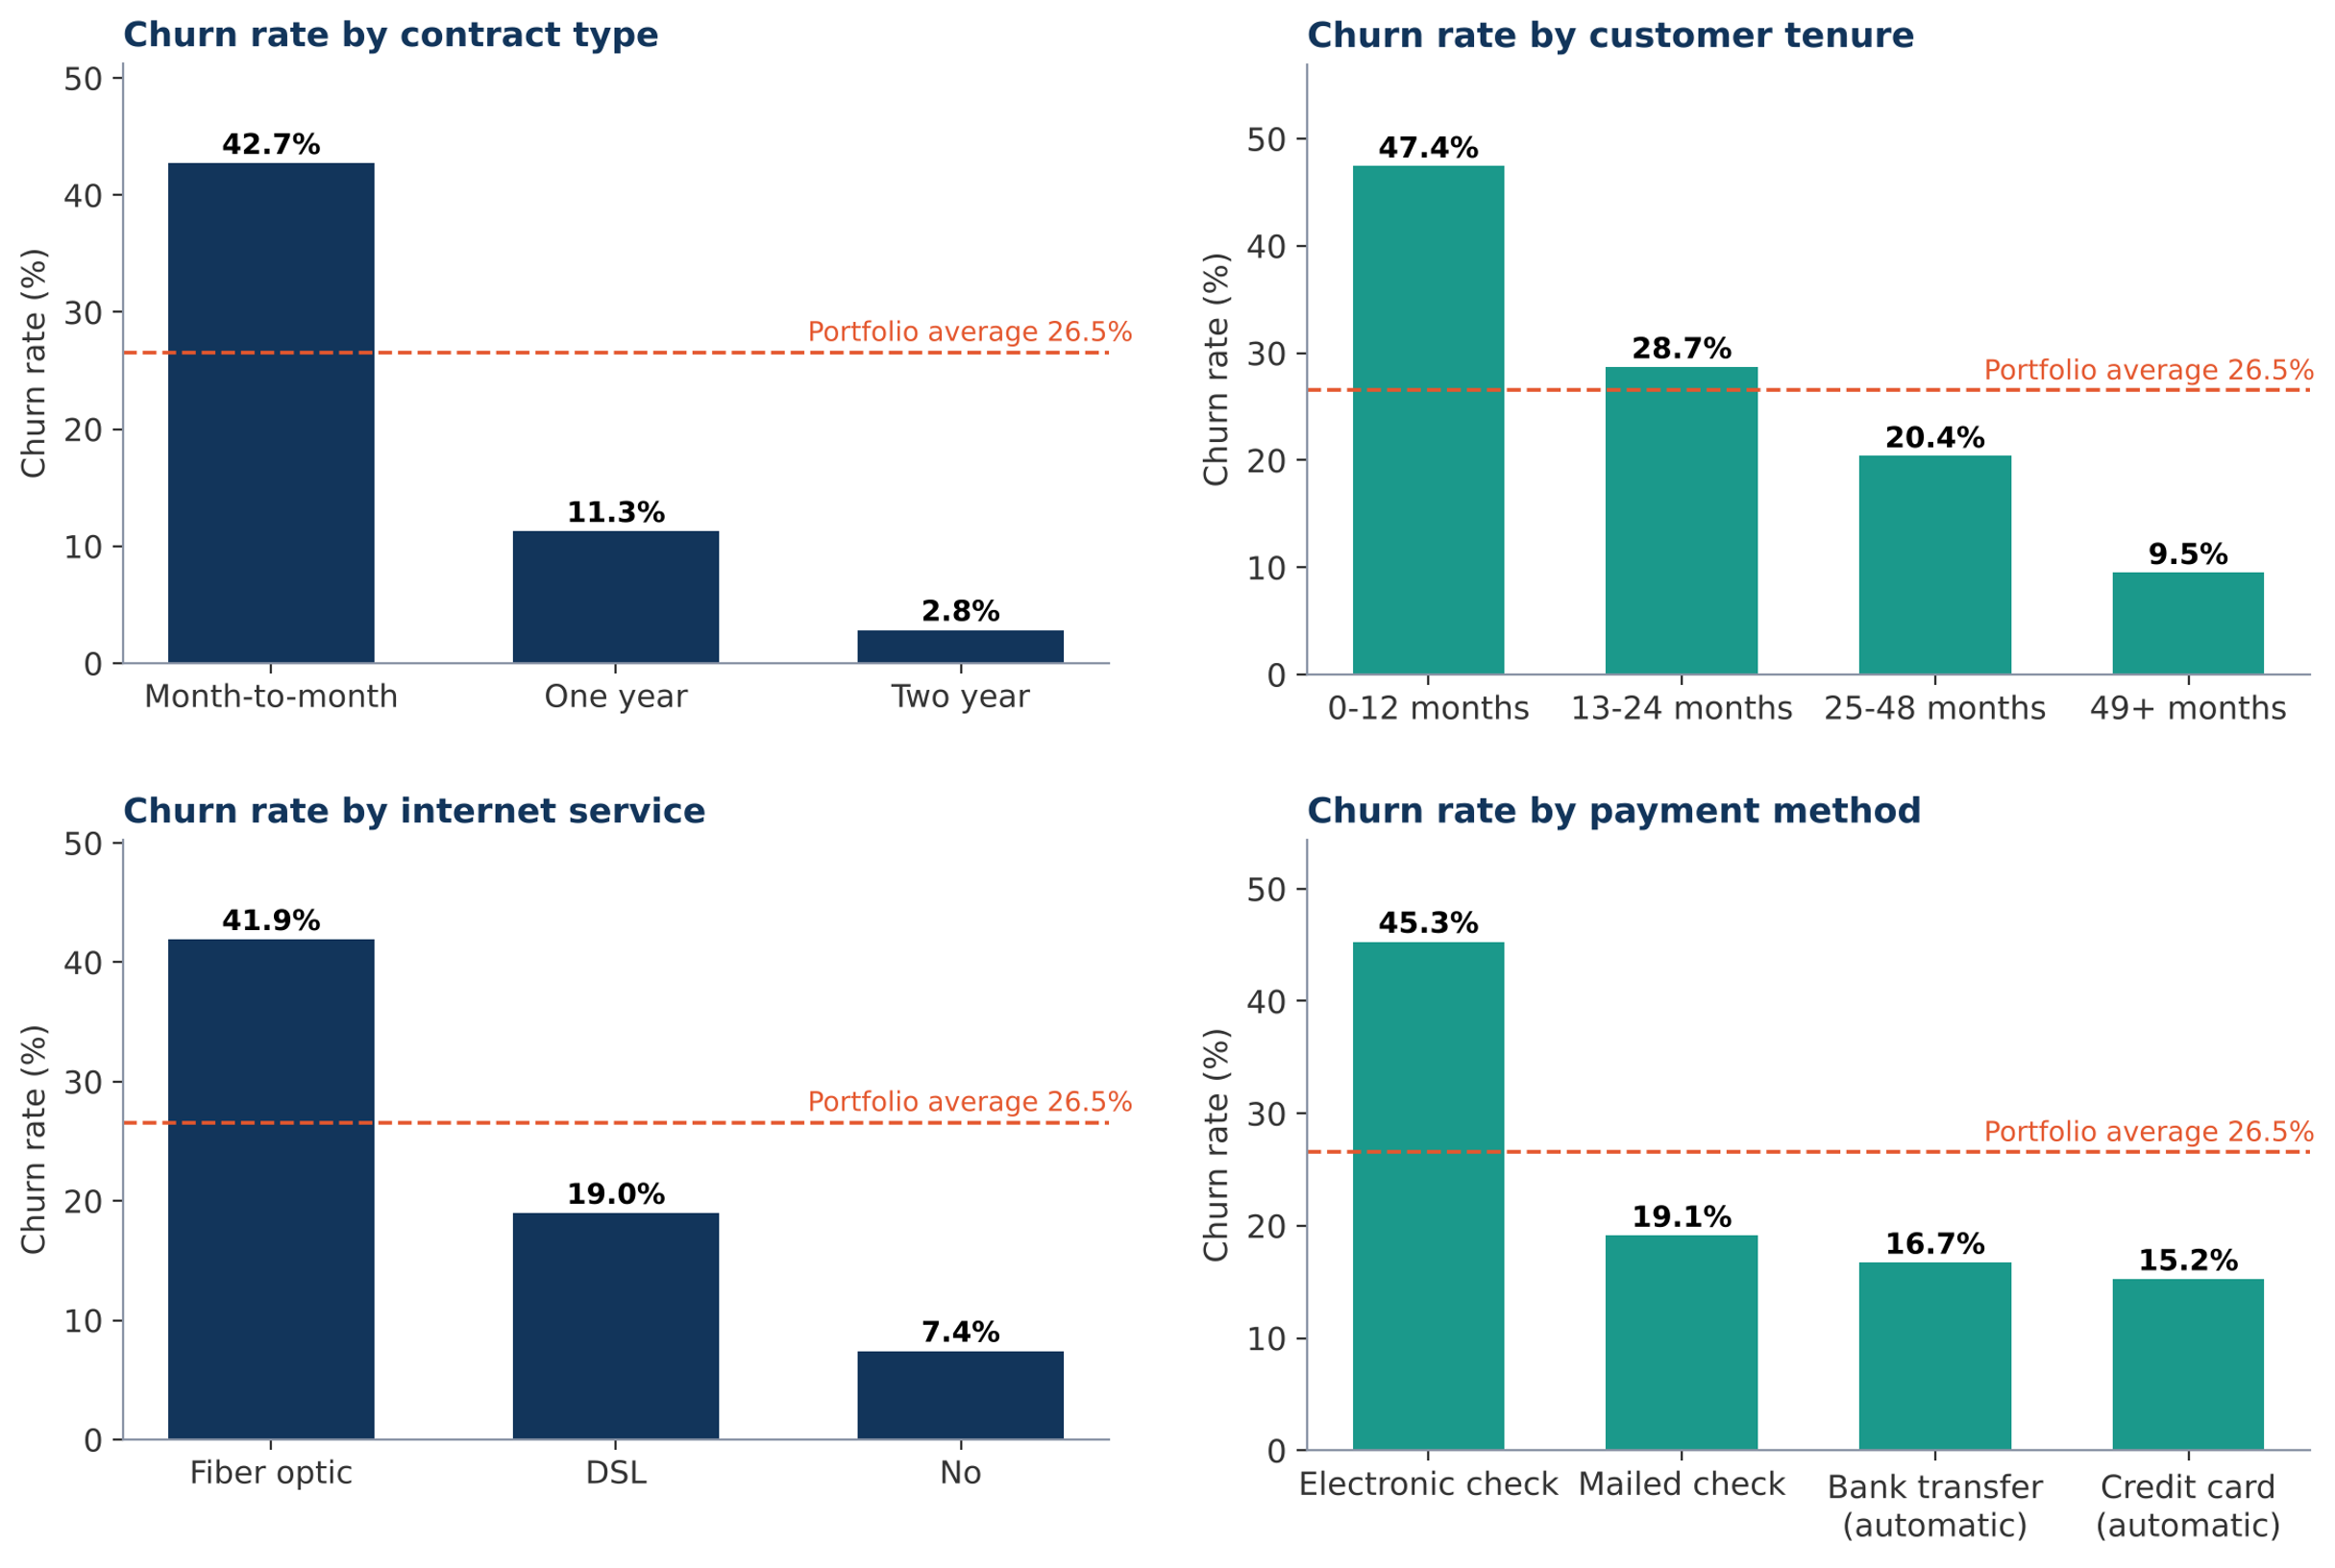
\includegraphics[width=0.92\linewidth,height=0.34\textheight,keepaspectratio]{./media/34b68642808fe15a12d9382791e84de83b0f9be5.png}

\emph{Figure 1: Churn rate by contract, tenure, internet service and
payment method (dashed line = 26.5\% portfolio average)}

\begin{itemize}
\item
  \textbf{Contract:} month-to-month customers churn at 42.7\%, against
  11.3\% on one-year and 2.8\% on two-year contracts. They are 88.6\% of
  all churners (1,655 of 1,869).
\item
  \textbf{Tenure:} 47.4\% of customers in their first 12 months churn,
  against 9.5\% after 48 months.
\item
  \textbf{Internet service:} fiber optic customers churn at 41.9\%
  against 19.0\% for DSL, and they also pay the most (USD 91.50 a month
  on average).
\item
  \textbf{Payment method:} electronic-check payers churn at 45.3\%; the
  other three methods sit between 15.2\% and 19.1\%.
\item
  \textbf{Protective add-ons:} among internet customers, those with both
  Online Security and Tech Support churn at 9.0\%, against 49.0\% for
  those with neither.
\end{itemize}

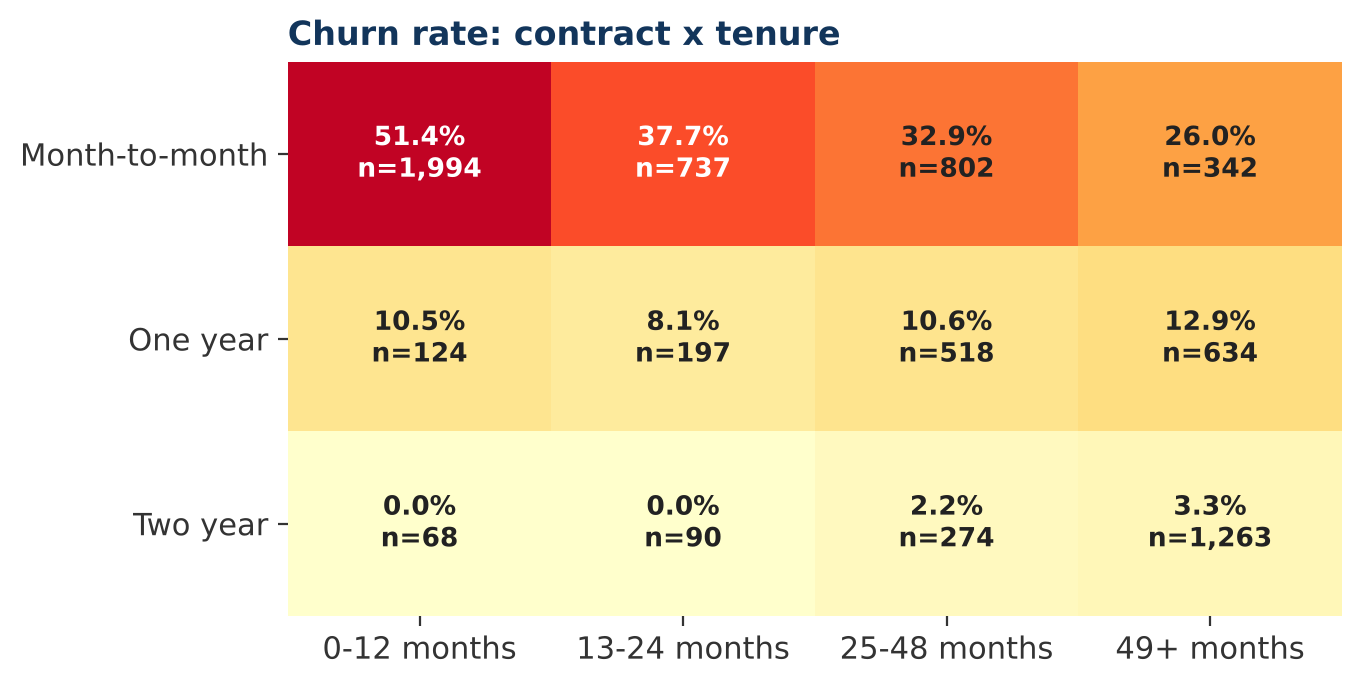
\includegraphics[width=0.92\linewidth,height=0.34\textheight,keepaspectratio]{./media/16efd039e0b76259f76926a6e29f79977e2704c6.png}

\emph{Figure 2: Churn rate by contract and tenure band (n = customers in
each cell)}

The worst segment is month-to-month, fiber optic customers in their
first year: 916 customers, 70.2\% churn, USD 75,183 of monthly revenue.
The 0.0\% cells for two-year contracts rest on small groups (n = 68 and
90), so we read them as "very low", not "zero".

The table lists the eleven queries and the technique each one
demonstrates.

\begin{longtable}[]{@{}
  >{\raggedright\arraybackslash}p{(\columnwidth - 4\tabcolsep) * \real{0.3324}}
  >{\raggedright\arraybackslash}p{(\columnwidth - 4\tabcolsep) * \real{0.2991}}
  >{\raggedright\arraybackslash}p{(\columnwidth - 4\tabcolsep) * \real{0.3685}}@{}}
\toprule\noalign{}
\begin{minipage}[b]{\linewidth}\raggedright
\textbf{Query}
\end{minipage} & \begin{minipage}[b]{\linewidth}\raggedright
\textbf{SQL technique}
\end{minipage} & \begin{minipage}[b]{\linewidth}\raggedright
\textbf{Business question}
\end{minipage} \\
\midrule\noalign{}
\endhead
\bottomrule\noalign{}
\endlastfoot
portfolio\_kpis & Aggregates & What is the headline churn rate and
revenue lost? \\
churn\_by\_contract & GROUP BY, scalar subquery & Which contract carries
the churn, and what share of the total? \\
churn\_by\_tenure\_band & CASE band in view, GROUP BY & When do
customers leave? \\
churn\_by\_internet\_service, churn\_by\_payment\_method & JOIN via
view, GROUP BY & Which products and payment methods carry risk? \\
churn\_by\_support\_addons & WHERE, CASE, GROUP BY & Do protective
add-ons reduce churn? \\
high\_risk\_segments & GROUP BY, HAVING (at least 100 customers) & Which
segments should we target first? \\
churn\_vs\_portfolio\_average & CTE, RANK() window function & How far is
each segment from the average? \\
risk\_tier\_summary & JOIN to model scores & Do the
model\textquotesingle s tiers match what happened? \\
top\_at\_risk\_customers & JOIN, WHERE, ORDER BY & Who should agents
call first (active customers only)? \\
active\_base\_by\_tier & Filtered GROUP BY & How much revenue sits in
each tier of the live base? \\
\end{longtable}

\section{Churn model}

A logistic regression ranks customers well (ROC-AUC 0.845 on held-out
data) and its risk tiers behave as intended: the higher the tier, the
more customers actually left.

The model uses 17 inputs (tenure, monthly charges and 15 categorical
fields on services, contract and billing). We excluded gender, which has
no business use, and TotalCharges, which is roughly tenure times monthly
charge and made coefficients misleading; dropping it moved ROC-AUC by
less than 0.002. We held out 25\% of customers (1,761) for testing and
compared the model with a gradient-boosting challenger.

\begin{longtable}[]{@{}
  >{\raggedright\arraybackslash}p{(\columnwidth - 4\tabcolsep) * \real{0.4460}}
  >{\raggedright\arraybackslash}p{(\columnwidth - 4\tabcolsep) * \real{0.2770}}
  >{\raggedright\arraybackslash}p{(\columnwidth - 4\tabcolsep) * \real{0.2770}}@{}}
\toprule\noalign{}
\begin{minipage}[b]{\linewidth}\raggedright
\textbf{Hold-out metric}
\end{minipage} & \begin{minipage}[b]{\linewidth}\raggedright
\textbf{Logistic regression}
\end{minipage} & \begin{minipage}[b]{\linewidth}\raggedright
\textbf{Gradient boosting}
\end{minipage} \\
\midrule\noalign{}
\endhead
\bottomrule\noalign{}
\endlastfoot
ROC-AUC & 0.845 & 0.844 \\
PR-AUC & 0.635 & 0.653 \\
Brier score (lower is better) & 0.137 & 0.136 \\
Precision at 0.5 & 64.7\% & 66.7\% \\
Recall at 0.5 & 54.8\% & 48.4\% \\
Top-decile lift (baseline churn 26.5\%) & 2.76x & 2.89x \\
\end{longtable}

The two models are effectively tied, so we keep logistic regression:
every prediction can be broken into reasons that an agent can read out.
Scores stored in the database are out-of-fold (5-fold cross-validation,
ROC-AUC 0.843), so each customer is scored by a model that never saw
them.

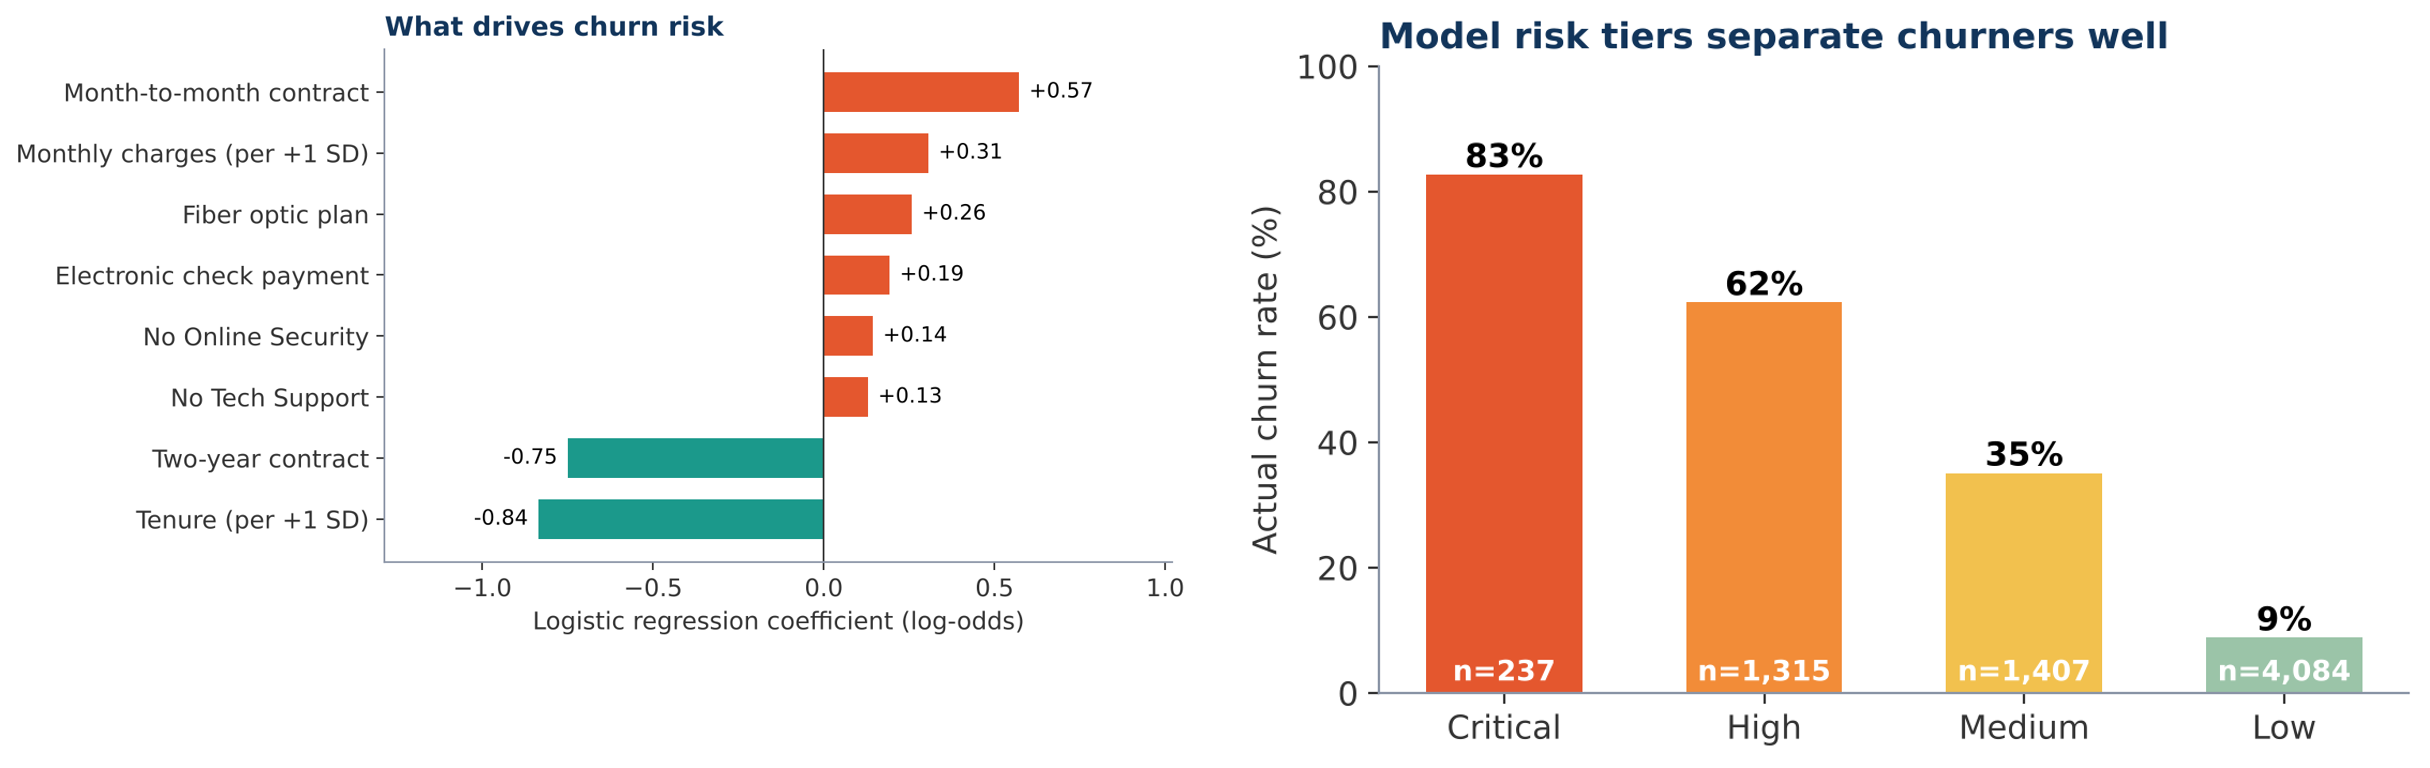
\includegraphics[width=0.92\linewidth,height=0.34\textheight,keepaspectratio]{./media/dfac6e39e0e494707a29c47fd4bf2fc0f400bc44.png}

\emph{Figure 3: Left, model drivers (log-odds; positive raises risk).
Right, actual churn rate by risk tier (n = customers per tier)}

Risk tiers cut the predicted probability at 0.25, 0.50 and 0.75. Actual
churn was 8.8\% in Low (4,084 customers), 35.1\% in Medium (1,407),
62.3\% in High (1,315) and 82.7\% in Critical (237). Flagging High and
Critical flags 1,552 customers (22.0\% of the base), captures 54.3\% of
all churners and is right 65.4\% of the time.

The drivers match the SQL findings. A month-to-month contract (+0.57),
higher monthly charges (+0.31 per standard deviation), fiber optic
(+0.26), electronic-check payment (+0.19) and missing Online Security or
Tech Support (+0.14, +0.13) raise risk. Longer tenure (-0.84 per
standard deviation) and a two-year contract (-0.75) lower it. For each
customer the model also lists the top three behavioural reasons for the
flag, computed as each factor\textquotesingle s effect against the
average customer. Demographic traits (senior citizen, partner,
dependents) are model inputs but are never shown as reasons.

\section{Dashboard}

The Streamlit dashboard turns the scored database into four working
views for the retention team. Every number is read from SQLite through
SQL, and by default the dashboard shows only customers who are still
active: 5,174 customers, of whom 537 are High or Critical, with USD
67,947 of monthly revenue expected to be at risk.

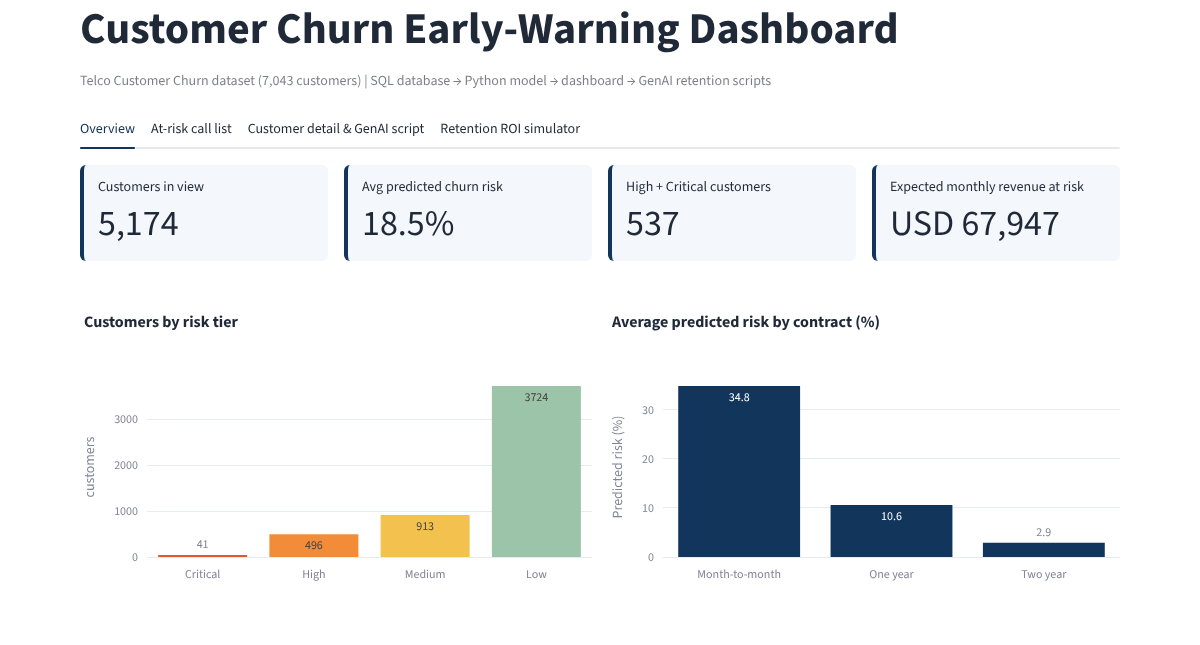
\includegraphics[width=0.92\linewidth,height=0.34\textheight,keepaspectratio]{./media/2dfeb9131c5d9fd749c9d44795a941d51b7f6f8e.png}

\emph{Figure 4: Overview tab with KPI tiles and risk-tier charts
(sidebar filters not shown)}

\begin{longtable}[]{@{}
  >{\raggedright\arraybackslash}p{(\columnwidth - 4\tabcolsep) * \real{0.2216}}
  >{\raggedright\arraybackslash}p{(\columnwidth - 4\tabcolsep) * \real{0.3878}}
  >{\raggedright\arraybackslash}p{(\columnwidth - 4\tabcolsep) * \real{0.3906}}@{}}
\toprule\noalign{}
\begin{minipage}[b]{\linewidth}\raggedright
\textbf{Tab}
\end{minipage} & \begin{minipage}[b]{\linewidth}\raggedright
\textbf{What the user sees}
\end{minipage} & \begin{minipage}[b]{\linewidth}\raggedright
\textbf{What the user can do}
\end{minipage} \\
\midrule\noalign{}
\endhead
\bottomrule\noalign{}
\endlastfoot
Overview & KPI tiles, customers by risk tier, average risk by contract,
highest-risk segments & Filter by contract, internet service and tenure
band; switch between active customers and all customers (back-test) \\
At-risk call list & Customers ranked by expected monthly loss (churn
probability x monthly charge) with the top three reasons & Choose risk
tiers; download the list as CSV \\
Customer detail and GenAI script & Churn probability, tier, contract
facts and why the customer was flagged & Pick a customer, generate an
editable call script and see its verification result \\
Retention ROI simulator & Customers contacted, expected churners
reached, expected saves, net benefit, ROI and a net-benefit curve & Move
the contact threshold, cost per contact, save rate, months of revenue
kept and discount cost \\
\end{longtable}

We tested the app with an automated headless run that opens every tab,
toggles the filters and clicks the script button; it finished with no
errors.

\section{GenAI assistant and verification}

The assistant drafts a short call script for each flagged customer, and
deterministic rules check it before an agent sees it. The AI therefore
never decides which offer to make or what a price is; it only words
facts and offers that the business has already approved.

\begin{enumerate}
\def\labelenumi{\arabic{enumi}.}
\item
  \textbf{Offer selection (rules, not AI).} Month-to-month customers get
  a 10\% discount for 12 months on a one-year contract; electronic-check
  payers get a waived paper-bill fee plus a one-off USD 5 credit for
  automatic payment; internet customers without Tech Support or Online
  Security get 3 months free; otherwise a free plan review. At most two
  offers are used.
\item
  \textbf{Prompt with approved facts only.} The model receives tenure,
  contract, internet plan, current monthly bill and the approved offers,
  plus rules: 80-130 words, no mention of churn, risk or scores, no
  personal traits, no invented prices or deadlines, and a closing
  question.
\item
  \textbf{Generation.} The script is written by Claude through the
  Anthropic API when a key is set, and by a deterministic template when
  offline, so the workflow always runs.
\item
  \textbf{Verification and human review.} The dashboard shows
  "Verification passed" or "Needs human review" with the reasons, and
  the agent can edit the text before use. Names are placeholders for the
  agent to fill in.
\end{enumerate}

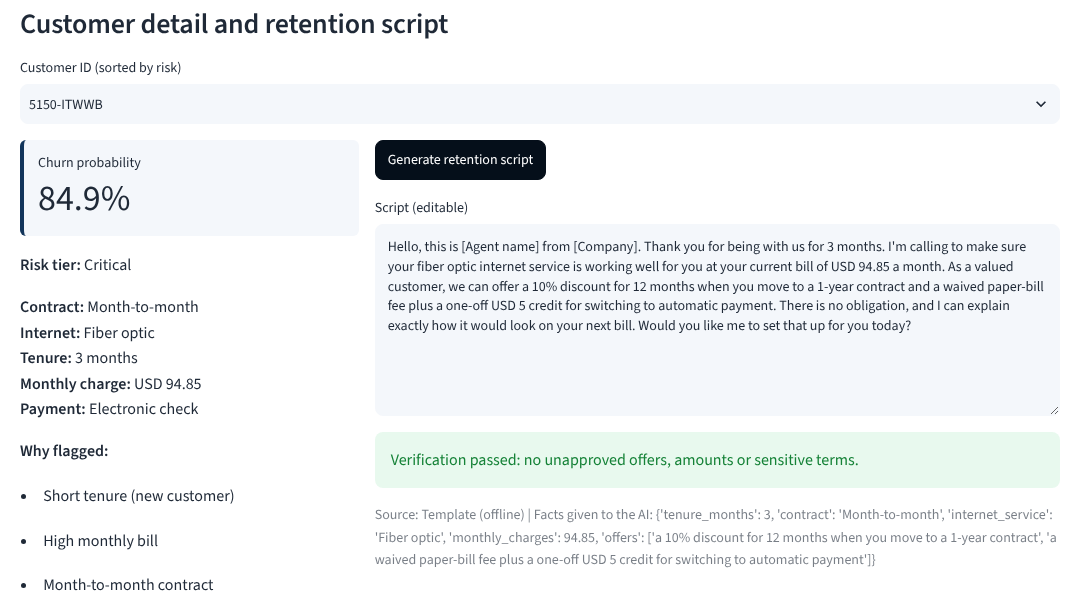
\includegraphics[width=0.92\linewidth,height=0.34\textheight,keepaspectratio]{./media/6fd2107ab1d0b9384386851da18abb61ba50b5d8.png}

\emph{Figure 5: Customer detail tab with the reasons for the flag, an
editable script and the verification result}

\begin{longtable}[]{@{}
  >{\raggedright\arraybackslash}p{(\columnwidth - 4\tabcolsep) * \real{0.2437}}
  >{\raggedright\arraybackslash}p{(\columnwidth - 4\tabcolsep) * \real{0.4350}}
  >{\raggedright\arraybackslash}p{(\columnwidth - 4\tabcolsep) * \real{0.3213}}@{}}
\toprule\noalign{}
\begin{minipage}[b]{\linewidth}\raggedright
\textbf{AI risk}
\end{minipage} & \begin{minipage}[b]{\linewidth}\raggedright
\textbf{Control in code}
\end{minipage} & \begin{minipage}[b]{\linewidth}\raggedright
\textbf{Evidence}
\end{minipage} \\
\midrule\noalign{}
\endhead
\bottomrule\noalign{}
\endlastfoot
Invented discounts, prices or durations & Every USD amount, percentage
and number of months must match the customer\textquotesingle s real
bill, real tenure or the approved offer list & Test scripts with a 50\%
discount or an unapproved price are rejected \\
Sensitive or inappropriate wording & Forbidden-term check (churn,
probability, scores, age, gender, family status) & A script mentioning a
"senior customer" is rejected \\
Off-brief output & Length 60-150 words, must mention an approved offer,
must end with a question & A script with no call to action is
rejected \\
LLM output fails the checks & The text is replaced by the template and
labelled as such & Failure path covered in code \\
Our own mistakes & Seven automated tests (verifier and database
integrity) & All 7 pass; all 7,043 template scripts pass the verifier \\
\end{longtable}

The model\textquotesingle s numbers are verified separately: row counts
are reconciled at every load step, the score table must cover every
customer with probabilities between 0 and 1, and every figure in this
report was taken from the pipeline\textquotesingle s output files
(summary.json and the sql\_results folder) and checked against them.

\section{Business impact}

Contacting the 537 active High and Critical customers is the best-value
starting point: an estimated USD 84,372 net benefit at a 596\% return,
under the assumptions below. The simulation applies only to customers
who are still active, because a customer who has already left cannot be
saved.

Assumptions (all editable in the dashboard): each contact costs USD 8;
30\% of contacted would-be churners are saved; a saved customer keeps 12
months of revenue; the retention discount costs 10\% of the revenue
kept. For each customer, expected benefit = churn probability x save
rate x monthly charge x 12 months; a customer is worth contacting when
that exceeds the contact cost plus the discount.

\begin{longtable}[]{@{}
  >{\raggedright\arraybackslash}p{(\columnwidth - 10\tabcolsep) * \real{0.1662}}
  >{\raggedright\arraybackslash}p{(\columnwidth - 10\tabcolsep) * \real{0.1828}}
  >{\raggedright\arraybackslash}p{(\columnwidth - 10\tabcolsep) * \real{0.1662}}
  >{\raggedright\arraybackslash}p{(\columnwidth - 10\tabcolsep) * \real{0.1551}}
  >{\raggedright\arraybackslash}p{(\columnwidth - 10\tabcolsep) * \real{0.2189}}
  >{\raggedright\arraybackslash}p{(\columnwidth - 10\tabcolsep) * \real{0.1108}}@{}}
\toprule\noalign{}
\begin{minipage}[b]{\linewidth}\raggedright
\textbf{Risk tier}
\end{minipage} & \begin{minipage}[b]{\linewidth}\raggedright
\textbf{Active customers}
\end{minipage} & \begin{minipage}[b]{\linewidth}\raggedright
\textbf{Expected saves}
\end{minipage} & \begin{minipage}[b]{\linewidth}\raggedright
\textbf{Cost (USD)}
\end{minipage} & \begin{minipage}[b]{\linewidth}\raggedright
\textbf{Net benefit (USD)}
\end{minipage} & \begin{minipage}[b]{\linewidth}\raggedright
\textbf{ROI}
\end{minipage} \\
\midrule\noalign{}
\endhead
\bottomrule\noalign{}
\endlastfoot
Critical & 41 & 9.6 & 1,352 & 8,890 & 657\% \\
High & 496 & 90.9 & 12,796 & 75,482 & 590\% \\
Medium & 913 & 98.6 & 15,582 & 67,194 & 431\% \\
Low & 3,724 & 88.4 & 36,123 & 27,191 & 75\% \\
\end{longtable}

The recommendation is to call Critical and High first, add Medium as
agent capacity allows, and serve the Low tier with low-cost automated
messages, because its return (75\%) is a fraction of the others.

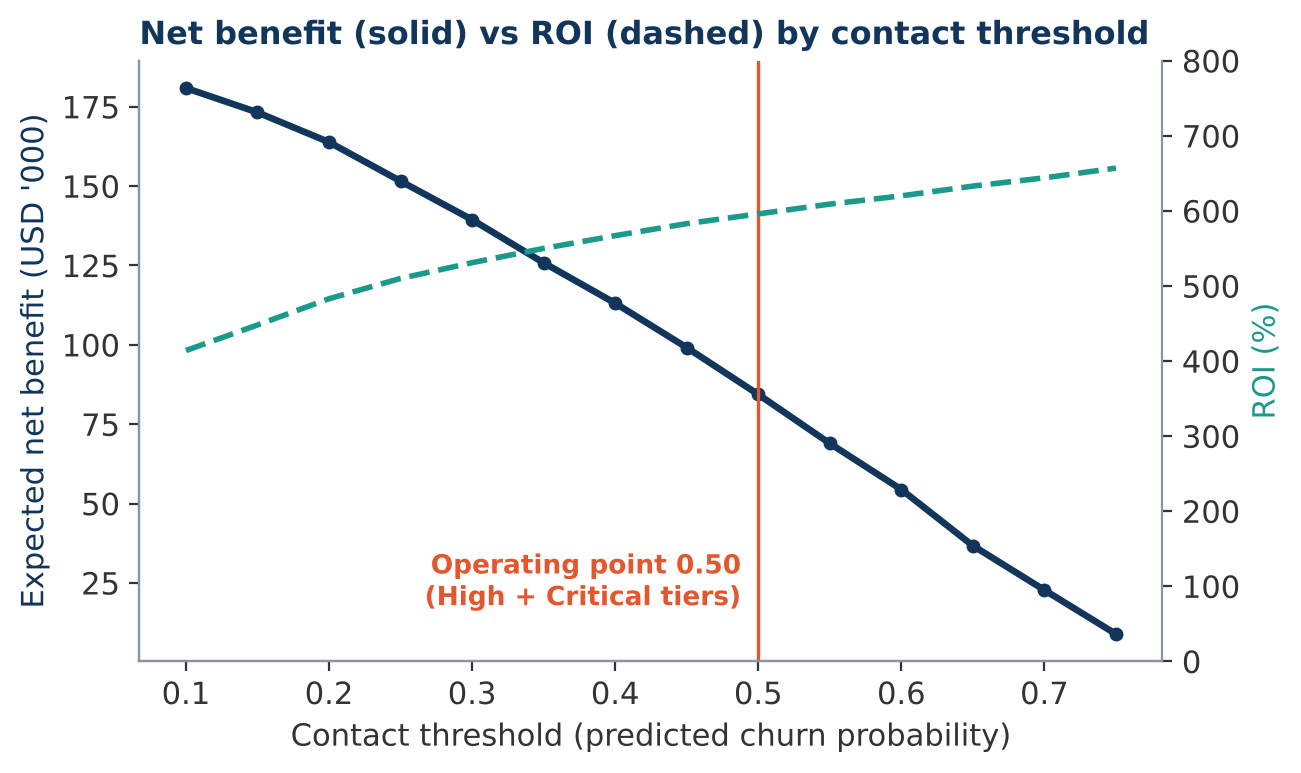
\includegraphics[width=0.92\linewidth,height=0.34\textheight,keepaspectratio]{./media/15dedfdb467d88ea31c1ba588e5048d758e3ac89.png}

\emph{Figure 6: Expected net benefit (solid) and ROI (dashed) as the
contact threshold moves; raising the threshold lifts ROI but reduces
total value}

The result depends most on the save rate, which we have assumed, not
measured. The campaign stays profitable even if only one in ten
contacted churners is saved.

\begin{longtable}[]{@{}
  >{\raggedright\arraybackslash}p{(\columnwidth - 6\tabcolsep) * \real{0.2216}}
  >{\raggedright\arraybackslash}p{(\columnwidth - 6\tabcolsep) * \real{0.2548}}
  >{\raggedright\arraybackslash}p{(\columnwidth - 6\tabcolsep) * \real{0.3020}}
  >{\raggedright\arraybackslash}p{(\columnwidth - 6\tabcolsep) * \real{0.2216}}@{}}
\toprule\noalign{}
\begin{minipage}[b]{\linewidth}\raggedright
\textbf{Save rate}
\end{minipage} & \begin{minipage}[b]{\linewidth}\raggedright
\textbf{Expected saves}
\end{minipage} & \begin{minipage}[b]{\linewidth}\raggedright
\textbf{Net benefit (USD)}
\end{minipage} & \begin{minipage}[b]{\linewidth}\raggedright
\textbf{ROI}
\end{minipage} \\
\midrule\noalign{}
\endhead
\bottomrule\noalign{}
\endlastfoot
10\% & 33.5 & 25,260 & 333\% \\
20\% & 67.0 & 54,816 & 505\% \\
30\% & 100.5 & 84,372 & 596\% \\
\end{longtable}

\section{Limitations and next steps}

We kept the scope deliberately narrow: one use case, one dataset, one
model, one dashboard and one AI feature, each tested, so the workflow
from data to insight is clear and explainable. The main limits are:

\begin{itemize}
\item
  \textbf{Snapshot data.} The dataset has no dates, so scores show
  relative risk and the ROI tab is a decision-support simulation, not a
  forecast. Active customers have not left yet, and we treat their
  probabilities as forward-looking risk.
\item
  \textbf{Assumed economics.} Contact cost, save rate, months of revenue
  kept and discount cost are assumptions, not measurements.
\item
  \textbf{Industry proxy.} Telecom behaviour is a stand-in for banks and
  insurers; the model and offers must be retrained and recalibrated on
  the institution\textquotesingle s own data.
\item
  \textbf{GenAI scope.} The live LLM call is optional and was not
  exercised in our test run, which had no API key; the template path,
  the verifier and the fallback logic were tested. The verifier checks
  facts and wording but cannot judge tone, so agents read and edit every
  script.
\item
  \textbf{Fairness.} Gender is excluded and demographic traits are never
  shown or used in scripts, but contract and tenure patterns can still
  correlate with protected groups, so outcomes should be monitored by
  segment.
\end{itemize}

Next steps:

\begin{enumerate}
\def\labelenumi{\arabic{enumi}.}
\item
  Collect time-stamped data so the model predicts churn within the next
  30 days.
\item
  A/B test the scripts against a control group to measure the real save
  rate.
\item
  Add an uplift model to target customers who are persuadable, not only
  at risk.
\item
  Connect the database to the CRM so the call list refreshes nightly.
\end{enumerate}

\section{Reproducibility}

The whole workflow runs from the repository with a few commands, and the
README documents setup, design decisions, verification and limitations.

\texttt{pip install -r requirements.txt}

\texttt{python run\_pipeline.py} \hfill \emph{data $\rightarrow$ SQLite $\rightarrow$ model $\rightarrow$ analysis}

\texttt{streamlit run app/dashboard.py} \hfill \emph{open the dashboard}

\texttt{python -m pytest -q} \hfill \emph{7 tests}

\begin{longtable}[]{@{}
  >{\raggedright\arraybackslash}p{(\columnwidth - 2\tabcolsep) * \real{0.3988}}
  >{\raggedright\arraybackslash}p{(\columnwidth - 2\tabcolsep) * \real{0.6012}}@{}}
\toprule\noalign{}
\begin{minipage}[b]{\linewidth}\raggedright
\textbf{Path}
\end{minipage} & \begin{minipage}[b]{\linewidth}\raggedright
\textbf{Purpose}
\end{minipage} \\
\midrule\noalign{}
\endhead
\bottomrule\noalign{}
\endlastfoot
sql/01\_schema.sql, sql/02\_queries.sql & Tables, constraints, analysis
view and the eleven named queries \\
src/etl.py & Clean, validate and load the CSV into SQLite \\
src/model.py & Train, evaluate and score the model; write scores and
reasons back to SQL \\
src/roi.py & Retention campaign ROI logic, shared by the dashboard and
this report \\
src/genai.py & Prompt, script generation (LLM or template) and the
verification layer \\
src/analysis.py & Run the queries; produce figures and summary.json \\
app/dashboard.py & Streamlit dashboard \\
tests/ & Automated tests \\
outputs/ & metrics.json, summary.json, SQL result CSVs and figures \\
\end{longtable}

Each module is short and commented with the reasoning behind its design
choices, so the team can walk through its own code line by line.

\end{document}
